%=====================================================================
%  Arogya AI : A Safety-First, Evidence-Grounded Conversational System
%              for Early-Stage Health Guidance
%
%  Single-file source.  Both figures are drawn with TikZ, so there are
%  no image files to upload: compile this file on its own (pdfLaTeX).
%=====================================================================
\documentclass[conference]{IEEEtran}
\IEEEoverridecommandlockouts

\usepackage{cite}
\usepackage{amsmath,amssymb,amsfonts}
\usepackage{algorithm}
\usepackage{algpseudocode}
\usepackage{graphicx}
\usepackage{booktabs}
\usepackage{array}
\usepackage{textcomp}
\usepackage{url}
\usepackage{tikz}
\usetikzlibrary{arrows.meta,positioning,calc}

% Figures live in figures/ ; the second path lets them also sit next to
% this file, so uploading images to the Overleaf root still works.
\graphicspath{{figures/}{./}}

\hyphenation{Ayur-vedic con-ver-sa-tion-al}

% --- float placement -------------------------------------------------
% This paper carries 18 floats (10 figures, 7 tables, 1 algorithm), which
% is well past LaTeX's defaults; without these it reports "Too many
% unprocessed floats".
\setcounter{topnumber}{3}
\setcounter{bottomnumber}{2}
\setcounter{totalnumber}{5}
\renewcommand{\topfraction}{0.95}
\renewcommand{\bottomfraction}{0.60}
\renewcommand{\textfraction}{0.05}
\renewcommand{\floatpagefraction}{0.70}
\renewcommand{\dbltopfraction}{0.95}
\renewcommand{\dblfloatpagefraction}{0.70}
\setcounter{dbltopnumber}{2}

% --- small helpers ---------------------------------------------------
\newcommand{\capYes}{\checkmark}
\newcommand{\capNo}{$\times$}
\newcommand{\capPart}{$\circ$}
\newcommand{\degF}{$^{\circ}$F}
\newcommand{\code}[1]{\texttt{\small #1}}

\begin{document}

\title{Arogya AI: A Safety-First, Evidence-Grounded\\
Conversational System for Early-Stage Health Guidance}

\author{
\IEEEauthorblockN{Rishav Kumar\textsuperscript{$*$},
                  Anshuman Kumar\textsuperscript{$\dagger$},
                  Rahul Kumar\textsuperscript{$\ddagger$}}
\IEEEauthorblockA{\textit{School of Computer Science and Engineering}\\
\textit{Vellore Institute of Technology}, Vellore, India\\
\textsuperscript{$*$}23BCE0462 \quad
\textsuperscript{$\dagger$}23BCE0311 \quad
\textsuperscript{$\ddagger$}23BCE0246}
\and
\IEEEauthorblockN{Guide: Prof. Deepa K}
\IEEEauthorblockA{\textit{School of Computer Science and Engineering}\\
\textit{Vellore Institute of Technology}, Vellore, India}
}

\maketitle

%---------------------------------------------------------------- ABSTRACT
\begin{abstract}
Software for self-triage falls into two families whose weaknesses are
complementary. Menu-driven symptom checkers are transparent and safe, but
they cannot interpret an illness described in the patient's own words;
conversational large language models (LLMs) read free text well, but they
occasionally return answers which are wrong or unsafe, and they do so
without warning. We describe Arogya AI, a conversational health-guidance
system which borrows from both families while keeping the language model in
a supporting role. The system extracts structured symptoms from natural
language, ranks the probable conditions with a Multinomial Naive Bayes
classifier, and grounds every explanation in a curated knowledge base by
retrieval-augmented generation (RAG). A deterministic rule layer scans each
message for emergency red flags before any model is consulted, so that a
life-threatening presentation is never buried inside a differential, and the
predicted conditions are additionally mapped to non-prescriptive Ayurvedic
lifestyle guidance. A working prototype covers 41 conditions and 87 symptom
features, retrieves from an index of 81 passages, and answers in tens of
milliseconds per turn. When no language model is available the system falls
back to deterministic local logic and behaves in the same way. Arogya AI is
intended to inform, and not to diagnose.
\end{abstract}

\begin{IEEEkeywords}
natural language processing, retrieval-augmented generation, Naive Bayes,
clinical decision support, conversational AI, patient safety.
\end{IEEEkeywords}

%---------------------------------------------------------------- INTRO
\section{Introduction}

Checking one's own symptoms before visiting a clinic is now routine, and the
software people use for it sits at one of two extremes. Rule-based checkers
are predictable and can be tied directly to clinical guidelines, but an audit
of widely used tools by Semigran \textit{et al.} \cite{semigran} found them
inflexible and prone to over-triage, largely because a fixed questionnaire
cannot absorb the nuance of free text. Conversational systems built on LLMs
are far more natural and, on some patient-education tasks, come close to
clinicians \cite{ayers,singhal}. Their fluency, however, conceals an
intermittent tendency to produce answers which are confident and wrong
\cite{thiru}; the reported rates of problematic responses span roughly
21.6\%--43.2\% across the leading systems.

Our position is that a dependable early-guidance assistant should borrow
selectively from each of these families, and that the language model should
be the least trusted component of the system rather than its core. In Arogya
AI an LLM, when one is configured at all, assists only in reading messy input
and in phrasing output. The two decisions which carry risk, namely whether a
message resembles an emergency and which conditions are the more probable
ones, are taken by a deterministic safety layer and by a transparent
statistical classifier. Every step which touches the LLM has a local
fallback, so the assistant keeps working, and behaves in the same way, when
no model key is present.

\textbf{Summary of contributions.} The contributions of this work are the
following.
\begin{itemize}
\item A processing pipeline in which emergency detection is evaluated first
on every turn and cannot be overridden by any later stage.
\item An explainable prediction stage, which returns a probability-ranked
differential together with a stated reason and the passages retrieved in
support of it.
\item A holistic layer, pairing each predicted condition with curated
Ayurvedic diet and lifestyle guidance.
\item A working full-stack implementation, with measured latency and a
verified emergency-escalation path.
\end{itemize}

%---------------------------------------------------------------- RELATED
\section{Related Work}

Work published over 2025--26 follows a recognisable progression. Fixed
decision trees were succeeded by conversational LLM responders, which were
then reinforced with retrieval so that their claims could be checked, and the
most recent efforts explore autonomous multi-agent systems. The transformer
architecture \cite{vaswani} and the pre-trained encoders derived from it
\cite{bert} underpin this whole line of work, while sentence-level embeddings
\cite{sbert} are what make dense semantic retrieval practical.
Retrieval-augmented generation, introduced by Lewis \textit{et al.}
\cite{lewis}, since surveyed for general LLMs by Gao \textit{et al.}
\cite{gao} and benchmarked in the medical domain by Xiong \textit{et al.}
\cite{xiong}, is the common remedy for hallucination. Broader reviews chart
the adoption of machine learning in medicine \cite{topol,rajkomar}, and
recent studies place GPT-class models on medical examinations and challenge
problems \cite{thiru,nori}. One recurring observation motivates our design:
such models can match physicians on patient education and yet fall short on
complex decision-making, reported as 96.9\% against 98.0\% in one 2025
comparison, which favours grounded, safety-checked and human-in-the-loop
architectures. Table~\ref{tab:families} summarises the principal families and
positions the proposed system among them.

%---------------------------------------------------------------- TABLE I
\begin{table*}[t]
\caption{Comparison of medical-AI approaches and the position of Arogya AI}
\label{tab:families}
\centering
\footnotesize
\begin{tabular}{@{}p{0.055\linewidth} p{0.125\linewidth} p{0.275\linewidth} p{0.165\linewidth} p{0.215\linewidth}@{}}
\toprule
\textbf{Ref.} & \textbf{Family} & \textbf{Mechanism} & \textbf{Strengths} & \textbf{Weaknesses}\\
\midrule
\cite{shortliffe}, \cite{semigran} & Rule-based checkers &
Hand-authored decision trees mapping symptoms to conditions. &
Transparent; safe; guideline-bound. &
Inflexible; ignores free-text nuance; over-triages.\\[2pt]
\cite{ayers}, \cite{singhal} & Standard LLM chatbots &
Prompt-and-answer QA over patient questions. &
Fluent, empathetic dialogue. &
Hallucinates; lacks verifiable grounding.\\[2pt]
\cite{lewis}--\cite{xiong} & RAG-grounded LLMs &
Retrieve source passages, then generate. &
Lower hallucination; cites evidence. &
Added latency; quality bound to the corpus.\\[2pt]
\cite{thamma}, \cite{patel} & Agentic frameworks &
Multi-agent triage, diagnosis and planning. &
Proactive, multi-step reasoning. &
Costly; requires strict human oversight.\\[2pt]
\cite{khan}, \cite{alqarni} & Symptom ML/NLP &
Probabilistic classifiers over symptom sets. &
Lightweight and fast. &
Weak on conversation; no explanation.\\[2pt]
\cite{spec} & \textbf{Arogya AI (proposed)} &
Safety-first pipeline: dialogue, NB, RAG and Ayurveda. &
Grounded, explainable, holistic, private. &
Traditional-medicine corpus still expanding.\\
\bottomrule
\end{tabular}
\end{table*}

%---------------------------------------------------------------- PROPOSED
\section{Proposed System}

What distinguishes Arogya AI is less any individual module than the order in
which the modules are allowed to act. Six design choices follow from this.
The interface is genuinely conversational: the agent asks a small number of
targeted follow-up questions instead of requiring a complete form in advance.
Explanations are retrieved before they are written, so that factual claims
are anchored to controlled text rather than generated freely. No output is
presented as a verdict; each result carries a ranked differential, a
confidence value, and a visible trace of the stages which produced it.
Predicted conditions are mapped to curated Ayurvedic diet and lifestyle
notes, which acknowledges practices that many users already follow. A
rule-based emergency check precedes all of this and defers to human care as
soon as it fires. Finally, since the system needs neither a login nor
server-side storage, and supports both speech input and spoken output, it is
private and can be used hands-free.

%---------------------------------------------------------------- ARCH
\section{System Architecture}

A message travels from the chat window in the browser, over a REST interface,
to a FastAPI orchestrator which traverses a fixed sequence of stages
(Fig.~\ref{fig:pipeline}). The ordering is the one invariant of the design:
the red-flag scan is evaluated before every other stage on each turn, so an
emergency cannot be overridden later. The conversation state, together with
the symptoms accumulated so far, is persisted to a database row, so that
refreshing the page restores a session rather than discarding it. The
dialogue itself is governed by the finite-state machine of
Fig.~\ref{fig:fsm}. Each reply is accompanied by a trace of the stages which
ran, labelled \code{ok}, \code{skipped} or \code{triggered}, together with
the time each one took. Rendering this trace in the interface is what makes
the safety-first ordering and the RAG grounding directly observable.

%---------------------------------------------------------------- FIG 1
\begin{figure}[tb]
\centering
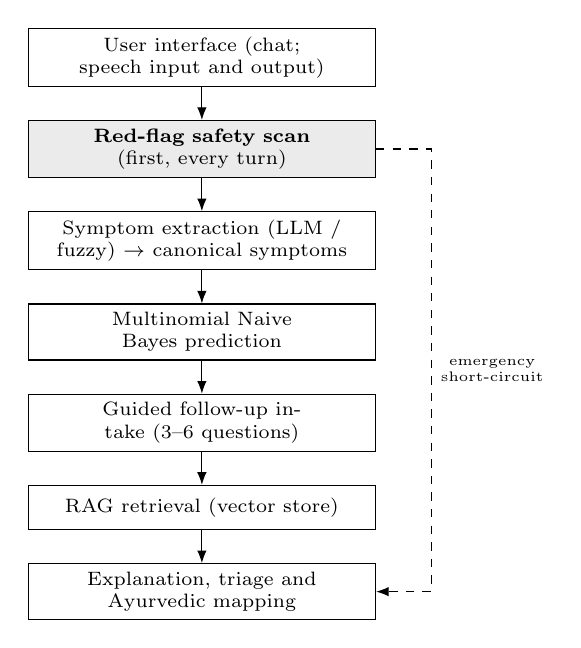
\begin{tikzpicture}[
  node distance=4.2mm,
  box/.style={draw, rectangle, align=center, inner sep=3pt,
              text width=42mm, font=\scriptsize, minimum height=5.6mm},
  ar/.style={-{Latex[length=1.6mm]}}
]
\node[box] (ui) {User interface (chat; speech input and output)};
\node[box, fill=black!8, below=of ui] (rf)
      {\textbf{Red-flag safety scan} (first, every turn)};
\node[box, below=of rf] (ex)
      {Symptom extraction (LLM / fuzzy) $\rightarrow$ canonical symptoms};
\node[box, below=of ex] (nb) {Multinomial Naive Bayes prediction};
\node[box, below=of nb] (fu) {Guided follow-up intake (3--6 questions)};
\node[box, below=of fu] (rg) {RAG retrieval (vector store)};
\node[box, below=of rg] (op) {Explanation, triage and Ayurvedic mapping};

\draw[ar] (ui) -- (rf);
\draw[ar] (rf) -- (ex);
\draw[ar] (ex) -- (nb);
\draw[ar] (nb) -- (fu);
\draw[ar] (fu) -- (rg);
\draw[ar] (rg) -- (op);

\coordinate (ra) at ($(rf.east)+(7mm,0)$);
\coordinate (rb) at ($(op.east)+(7mm,0)$);
\draw[ar, dashed] (rf.east) -- (ra) -- (rb)
      node[midway, right, font=\tiny, align=center]
      {emergency\\short-circuit} -- (op.east);
\end{tikzpicture}
\caption{The processing pipeline. A turn enters at the top and passes down
through the stages in the order shown. The red-flag scan is evaluated before
every other stage, and a match short-circuits the stages below it and routes
the turn directly to the emergency response.}
\label{fig:pipeline}
\end{figure}

%---------------------------------------------------------------- FIG 2
\begin{figure}[tb]
\centering
\resizebox{\columnwidth}{!}{%
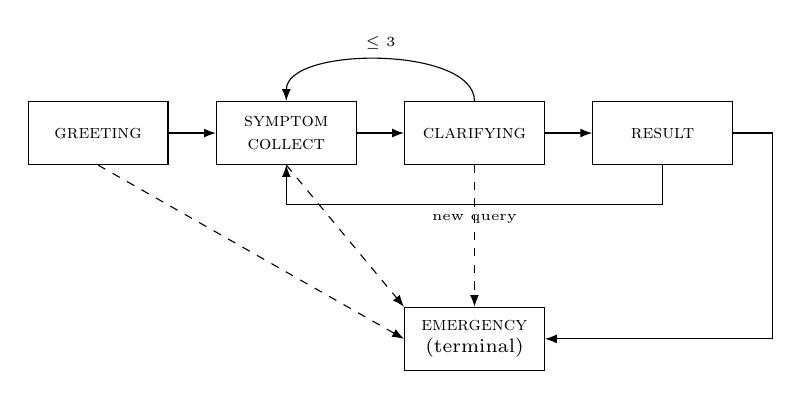
\begin{tikzpicture}[
  st/.style={draw, rectangle, align=center, font=\scriptsize,
             inner sep=2.5pt, minimum height=8mm, text width=16mm},
  ar/.style={-{Latex[length=1.5mm]}}
]
\node[st] (g)  {\textsc{greeting}};
\node[st, right=6mm of g]  (sc) {\textsc{symptom}\\\textsc{collect}};
\node[st, right=6mm of sc] (cl) {\textsc{clarifying}};
\node[st, right=6mm of cl] (rs) {\textsc{result}};
\node[st, below=18mm of cl] (em) {\textsc{emergency}\\(terminal)};

\draw[ar] (g)  -- (sc);
\draw[ar] (sc) -- (cl);
\draw[ar] (cl) -- (rs);

\draw[ar] (cl.north) .. controls +(0,7mm) and +(0,7mm) ..
      node[midway, above, font=\tiny] {$\leq 3$} (sc.north);

\draw[ar] (rs.south) -- ++(0,-5mm)
      -- node[midway, below, font=\tiny] {new query}
      ($(sc.south)+(0,-5mm)$) -- (sc.south);

\draw[ar, dashed] (g.south)  -- (em.west);
\draw[ar, dashed] (sc.south) -- (em.north west);
\draw[ar, dashed] (cl.south) -- (em.north);
\draw[ar]         (rs.east)  -- ++(5mm,0) |- (em.east);
\end{tikzpicture}}
\caption{The conversation states. The solid arrows along the top row are the
normal progression through a consultation; the loop out of
\textsc{clarifying} is taken at most three times before a result is produced,
and a result may be followed by a new query. The dashed arrows indicate that
a red-flag match can drive any state to the terminal \textsc{emergency}
state.}
\label{fig:fsm}
\end{figure}

%---------------------------------------------------------------- DATA
\section{Dataset and Preprocessing}

The classifier is trained on a symptom--disease table modelled on the
structure of the established public datasets, covering 41 conditions over an
87-dimensional binary symptom space. Converting a sentence into a vector of
that space proceeds in four steps. The text is first lower-cased, tokenised
and cleared of non-clinical filler words. A curated vocabulary then maps
colloquial phrasing onto canonical symptoms; ``loose motions'', for example,
is resolved to \code{diarrhea} and ``burning up'' to \code{high\_fever}. A
lightweight stemmer folds inflections, so that ``coughing'' and ``coughs''
both map to \code{cough}. A short left-context check finally removes any
symptom which the user explicitly denies, which is what prevents ``no fever''
from setting the fever feature. Answers to the follow-up questions are
encoded back into the same vector; a reported temperature above 102\,\degF,
for instance, sets \code{high\_fever}.

Note that the retrieval corpus is kept independent of the classifier. 41
short knowledge-base articles are chunked and embedded into a vector index of
81 passages, which is used for grounding and for nothing else.

%---------------------------------------------------------------- METHOD
\section{Methodology}

\subsection{Condition Ranking}

For a binary symptom vector $\mathbf{x}=(x_1,\dots,x_n)$ with $n=87$, the
Multinomial Naive Bayes decision is computed in log-space, which prevents
underflow:
\begin{equation}
\hat{c} \;=\; \arg\max_{c \in \mathcal{C}}
\Big[\log P(c) + \sum_{i=1}^{n} x_i \log P(t_i \mid c)\Big],
\end{equation}
over the 41 conditions $\mathcal{C}$, with Laplace-smoothed likelihoods
\begin{equation}
P(t_i \mid c) \;=\; \frac{N_{ci}+\alpha}{N_c+\alpha n},
\qquad \alpha = 1 .
\end{equation}
Normalising the exponentiated class scores gives the ranked differential
which is shown to the user. Naive Bayes was chosen deliberately rather than
by default: it is inexpensive and, unlike a neural predictor, its output can
be attributed to individual symptoms.

\subsection{Evidence Retrieval}

For the leading condition, the query is embedded with a sentence encoder
\cite{sbert} and compared with the passage embeddings by cosine similarity,
\begin{equation}
\mathrm{sim}(\mathbf{q},\mathbf{d}) \;=\;
\frac{\mathbf{q}\cdot\mathbf{d}}{\|\mathbf{q}\|\,\|\mathbf{d}\|},
\end{equation}
returning the top-$k$ passages scoped to that condition, which are what
anchor the explanation.

\subsection{Guided Intake and Triage}

A single confident message previously advanced straight to a result, and such
a result reads as a guess rather than as a consultation. The intake now
interleaves clinical slots, namely duration, intensity, trend, temperature,
recent exposure, and appetite or sleep, with discriminating symptoms chosen
by the model to separate its leading candidates; it asks a minimum of three
questions and a maximum of six. A triage score then combines the baseline
severity of the condition with these answers, where severe intensity, a long
duration, a worsening trend and high fever each add weight, and resolves to
one of \textit{self-care}, \textit{appointment within one to two days}, or
\textit{see a doctor today}. Algorithm~\ref{alg:turn} states the per-turn
logic.

%---------------------------------------------------------------- ALGORITHM
\begin{algorithm}[t]
\footnotesize
\caption{Per-turn orchestration (safety first)}
\label{alg:turn}
\begin{algorithmic}[1]
\Require message $m$, session $s$, bounds \textsc{min}$=3$, \textsc{max}$=6$
\State $sym \gets$ \textsc{ExtractSymptoms}($m$) \Comment{LLM, else fuzzy}
\State $s.sym \gets s.sym \cup sym$
\If{\textsc{RedFlag}($m$, $s.sym$)}
  \State \Return \textsc{Emergency}($pattern$) \Comment{overrides all}
\EndIf
\State $P \gets$ \textsc{NaiveBayes}($s.sym$) \Comment{Eq.~(1)}
\If{$s.asked <$ \textsc{min} \textbf{or} (\textsc{Ambiguous}($P$) \textbf{and} $s.asked <$ \textsc{max})}
  \State \Return \textsc{Clarifying}(\textsc{NextFollowup}($P,s$))
\EndIf
\State $E \gets$ \textsc{RagRetrieve}($P_1$, $s.sym$) \Comment{Eq.~(3)}
\State $t \gets$ \textsc{Triage}($P_1$, $s.slots$);\quad
       $a \gets$ \textsc{Ayurveda}($P_1$)
\State \Return \textsc{Result}($P$, $E$, $t$, $a$)
\end{algorithmic}
\end{algorithm}

%---------------------------------------------------------------- SAFETY
\section{Safety Layer}

The red-flag layer is expressed as deterministic rules and not as a model, so
that it cannot be argued out of firing. Because the classifier vocabulary and
the rule vocabulary were authored separately, an alias map connects them;
\code{breathlessness}, for example, is mapped to
\code{shortness\_of\_breath}. Note that without such a map, danger signs
mentioned across different turns would never accumulate into a rule match.
Table~\ref{tab:redflag} lists the eight categories which are monitored. When
a rule fires the conversation moves to the terminal \textsc{emergency} state,
in which no prediction is given at all and the user is directed to urgent
care and to the local emergency number.\footnote{Configurable; the deployment
defaults to 112/108 for India.}

%---------------------------------------------------------------- TABLE II
\begin{table}[t]
\caption{Emergency categories monitored by the safety layer}
\label{tab:redflag}
\centering
\footnotesize
\begin{tabular}{@{}p{0.23\linewidth} p{0.67\linewidth}@{}}
\toprule
\textbf{Category} & \textbf{Example trigger}\\
\midrule
Cardiac & Chest pain or pressure with arm/jaw pain, sweating, or
breathlessness.\\[1pt]
Stroke & Worst-ever headache, one-sided weakness, slurred speech, sudden
vision loss.\\[1pt]
Respiratory & Severe breathing difficulty; unable to finish a sentence; blue
lips or face.\\[1pt]
Bleeding & Uncontrolled bleeding; vomiting or coughing up blood.\\[1pt]
Anaphylaxis & Airway swelling together with difficulty breathing.\\[1pt]
Obstetric & Severe abdominal or pregnancy-related emergencies.\\[1pt]
Abdominal & Sudden, severe, or rigid-abdomen presentations.\\[1pt]
Mental health & Self-harm or crisis language.\\
\bottomrule
\end{tabular}
\end{table}

%---------------------------------------------------------------- IMPL
\section{Implementation}

The client is a single-page application written in React and TypeScript and
styled with Tailwind CSS. It provides a differential chart, triage and
Ayurveda cards, two-way voice (browser speech-to-text for input and
text-to-speech for output), a Markdown export of the consultation, and a
layout which reflows to phone width. The server is a FastAPI application over
SQLite, organised as an orchestrator state machine with a services layer
beneath it, and exposes REST endpoints for session creation, chat, history
retrieval, a consultation report, live model statistics and a health check.
Classification uses the Multinomial Naive Bayes implementation of
\code{scikit-learn} \cite{sklearn}, persisted with \code{joblib}; retrieval
uses a vector store with \code{sentence-transformers} embeddings
\cite{sbert}; and an OpenAI-compatible LLM is optional, and always sits
behind a fuzzy fallback. The deployment spans 41 conditions, 87 symptom
features, an index of 81 passages over 41 documents, eight red-flag
categories and 41 Ayurvedic entries. Fig.~\ref{fig:ui} shows the assembled
client at desktop width, and Fig.~\ref{fig:mobile} the same consultation
after the layout has reflowed to a phone.

Two engineering changes were needed before the system became interactive. The
sentence encoder is expensive to load, so it is warmed on a background thread
and the API begins serving at once instead of blocking for something like
half a minute. In addition, when no valid model key is configured, the
language-model calls return immediately rather than attempting a doomed
network request on every turn. Table~\ref{tab:latency} reports the resulting
improvements, and Fig.~\ref{fig:latency} plots them on a logarithmic scale.
Note that the two changes are independent: the first removes a fixed cost
paid once at startup, the second a cost paid again on every turn.

%---------------------------------------------------------------- FIG UI
\begin{figure*}[t]
\centering
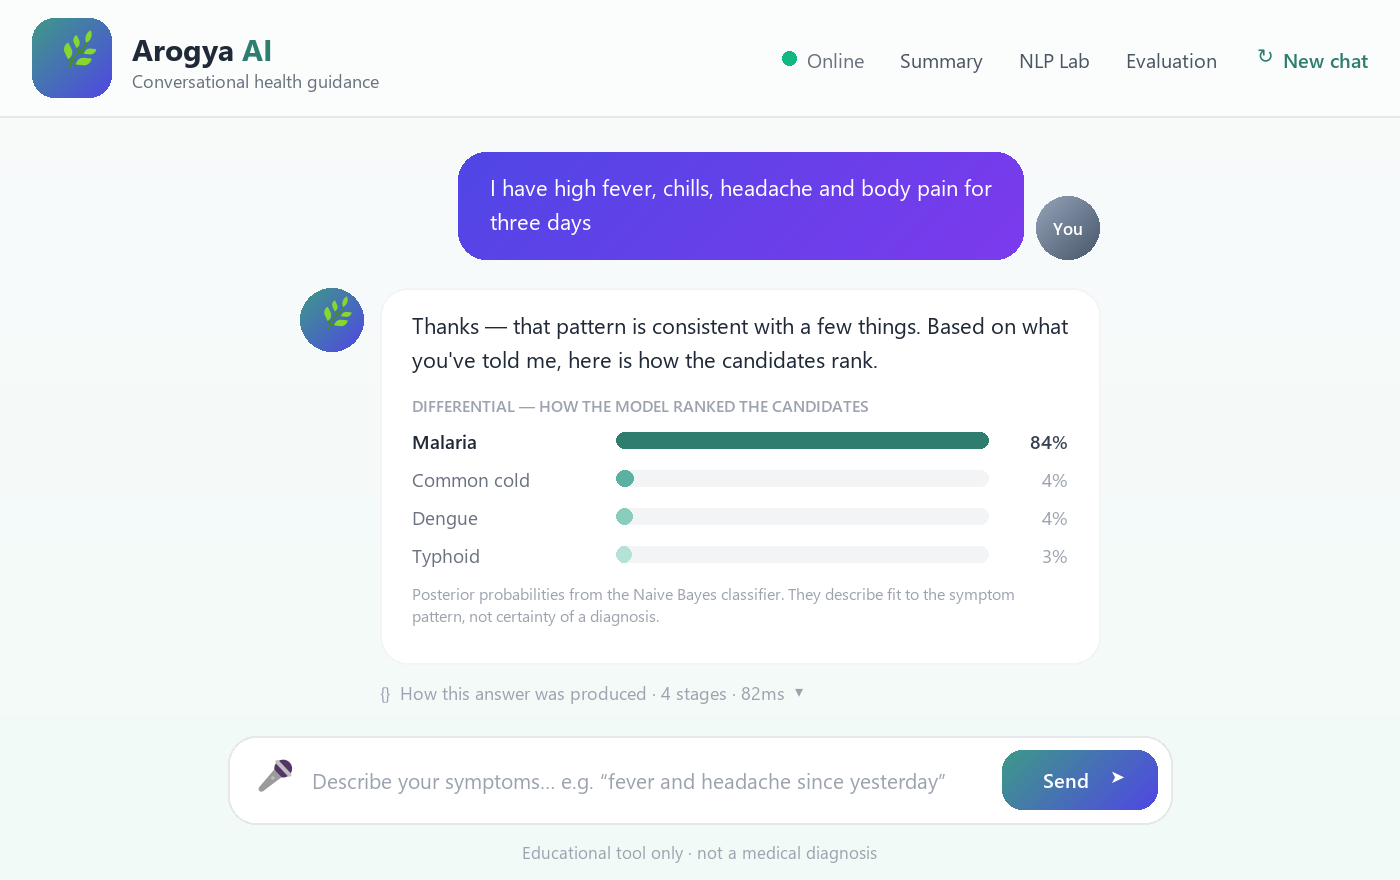
\includegraphics[width=0.86\textwidth]{screenshot_chat.png}
\caption{The client at desktop width, at the end of a consultation. The
user's message and the assistant's reply are shown in sequence, and the
ranked differential is drawn inside the reply, each candidate carrying its
posterior probability. The line beneath the reply expands into the per-turn
trace of Fig.~\ref{fig:tracess}. This figure and
Figs.~\ref{fig:result}--\ref{fig:mobile} are rendered from the client's own
components for one fixed example session.}
\label{fig:ui}
\end{figure*}

%---------------------------------------------------------------- FIG LATENCY
\begin{figure}[tb]
\centering
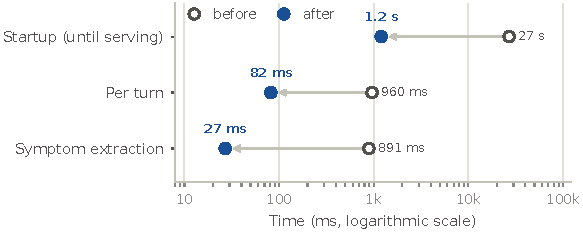
\includegraphics[width=\columnwidth]{fig_latency.pdf}
\caption{The effect of the two optimisations, plotted from
Table~\ref{tab:latency}. Hollow markers are the measurements before the
change and filled markers those after it; the arrow runs from one to the
other. The axis is logarithmic, since startup and per-turn costs differ by
more than two orders of magnitude.}
\label{fig:latency}
\end{figure}

%---------------------------------------------------------------- TABLE III
\begin{table}[t]
\caption{Latency before and after the two optimisations}
\label{tab:latency}
\centering
\footnotesize
\begin{tabular}{@{}l c c@{}}
\toprule
\textbf{Metric} & \textbf{Before} & \textbf{After}\\
\midrule
Startup (until serving) & $\sim$27\,s   & $\sim$1.2\,s\\
Per turn                & $\sim$960\,ms & $\sim$82\,ms\\
Symptom extraction      & 891\,ms       & 27\,ms\\
LLM fallback coverage   & ---           & 100\%\\
\bottomrule
\end{tabular}
\end{table}

%---------------------------------------------------------------- RESULTS
\section{Experimental Results}

For the input ``I have high fever, chills, headache and body pain for three
days'', the extractor recovered \code{high\_fever}, \code{fever},
\code{chills}, \code{headache}, \code{pain} and \code{shivering}; the safety
scan passed; Naive Bayes returned a ranked differential; and the intake asked
six short follow-up questions before presenting a result which bundled a
triage recommendation, a retrieved evidence source, Ayurvedic guidance, and a
list of symptoms to watch for. Fig.~\ref{fig:result} shows that result as the
user receives it. The end-to-end round trip took approximately one second.

To check the safety path we submitted the sentence ``severe crushing chest
pain spreading to my left arm, sweating and short of breath''. It was
intercepted before any prediction ran and was routed to the
\textsc{emergency} state, matching the cardiac pattern and replacing the
usual reply by an instruction to seek immediate care; Fig.~\ref{fig:emerg}
records the reply. Note that no differential appears in it at all, which is
the behaviour the safety layer is there to produce. This confirms that the
most safety-critical behaviour of the system depends neither on the
classifier nor on the language model. Table~\ref{tab:capability} contrasts
the system with the baseline families. Because the ranking is performed by a
probability model and the evidence is supplied by a retriever, the
differential and its sources can both be shown openly, which addresses the
transparency concern raised repeatedly in the literature.

%---------------------------------------------------------------- FIG RESULT
\begin{figure}[tb]
\centering
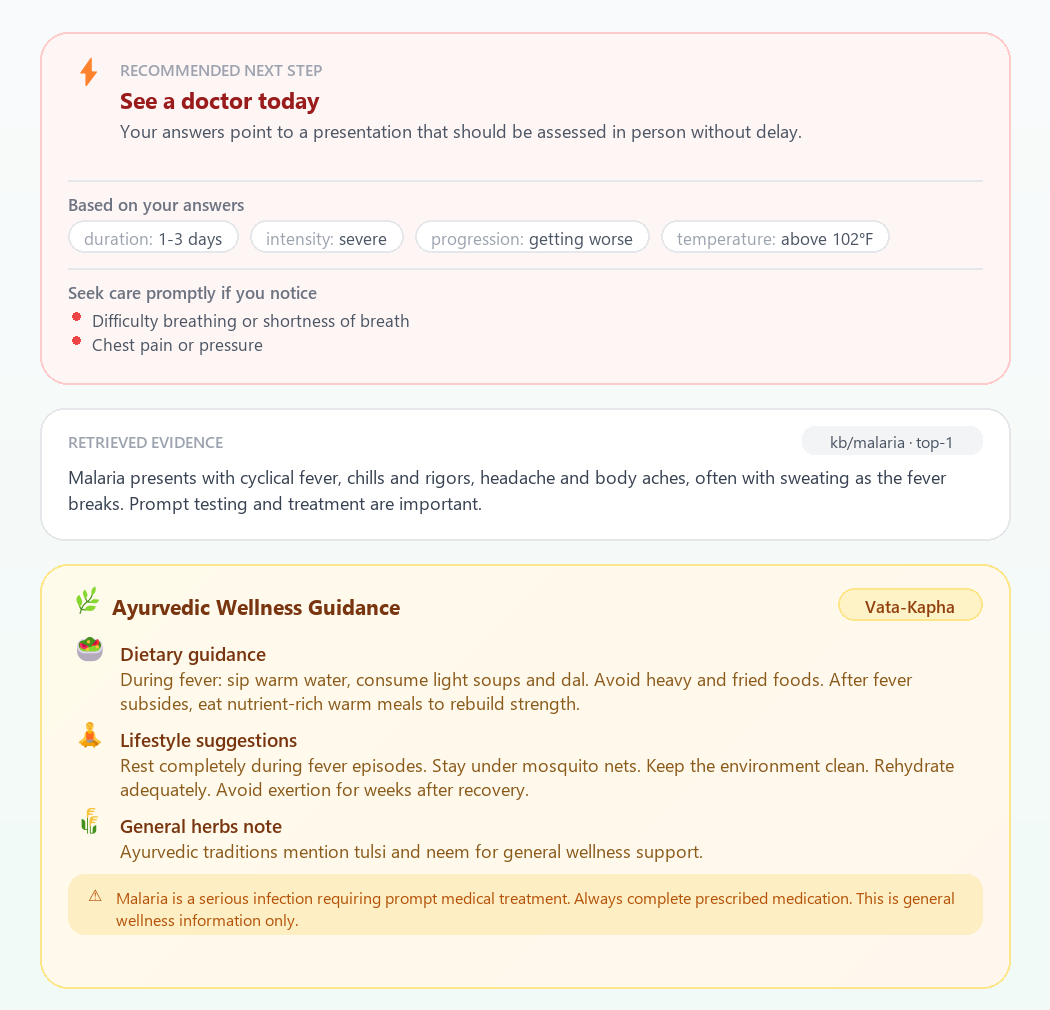
\includegraphics[width=0.92\columnwidth]{screenshot_result.png}
\caption{The result panel for the running example. The triage recommendation
is given first, together with the follow-up answers it was derived from and
the symptoms which should prompt the user to seek care sooner; beneath it sit
the passage retrieved for the leading condition and the curated Ayurvedic
guidance, which closes with its own caution note.}
\label{fig:result}
\end{figure}

%---------------------------------------------------------------- FIG EMERG
\begin{figure}[tb]
\centering
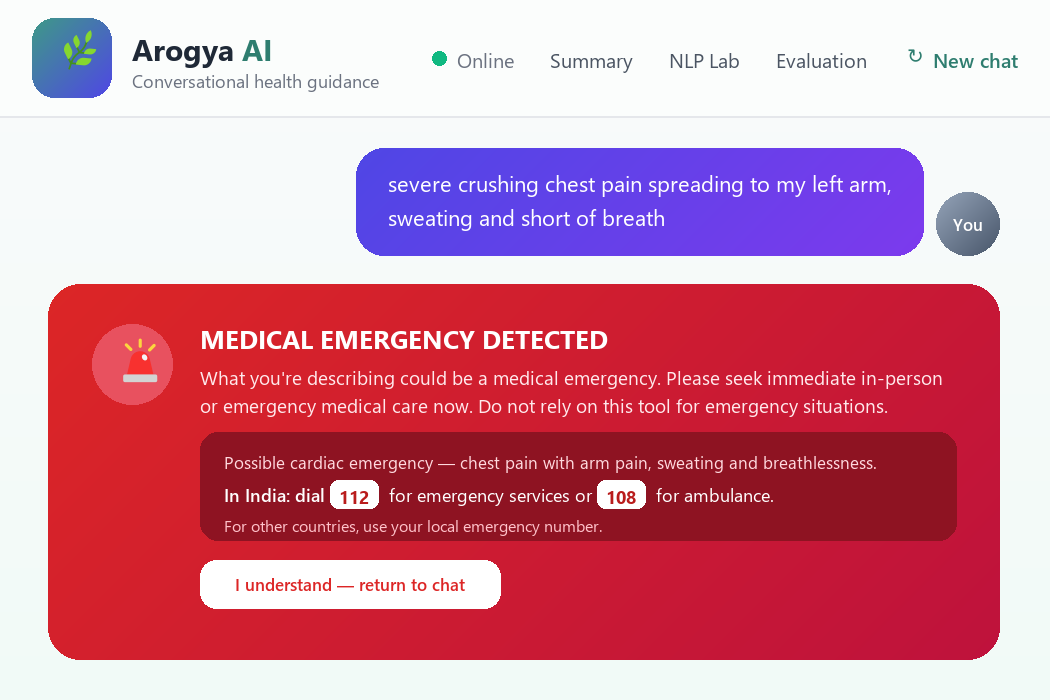
\includegraphics[width=\columnwidth]{screenshot_emergency.png}
\caption{The reply to the chest-pain test sentence. The red-flag scan matched
the cardiac pattern, so the conversation moved to the terminal
\textsc{emergency} state. Note that no differential appears anywhere in the
reply, because the prediction stage never ran; the user is directed to urgent
care and to the local emergency number instead.}
\label{fig:emerg}
\end{figure}

%---------------------------------------------------------------- FIG MOBILE
\begin{figure}[tb]
\centering
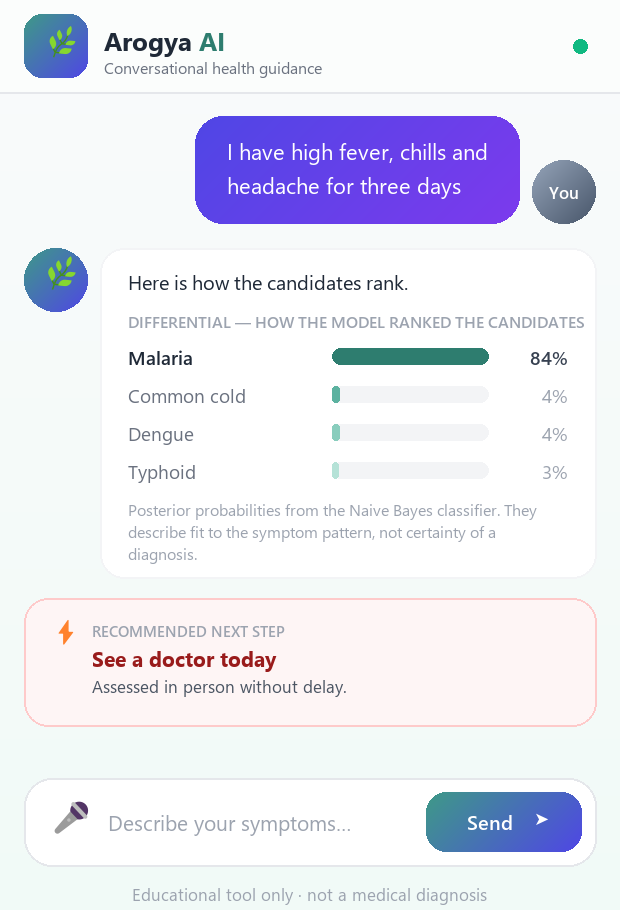
\includegraphics[height=0.33\textheight]{screenshot_mobile.png}
\caption{The same consultation at phone width. The differential and the
triage card stack into a single column, the header collapses to the logo and
the status dot, and the voice control stays in the composer, so the
assistant remains usable hands-free.}
\label{fig:mobile}
\end{figure}

%---------------------------------------------------------------- TABLE IV
\begin{table*}[t]
\caption{Capability comparison against baseline families
(\capYes: supported; \capPart: partial; \capNo: absent)}
\label{tab:capability}
\centering
\footnotesize
\begin{tabular}{@{}p{0.26\linewidth} c c c c c@{}}
\toprule
\textbf{Capability} & \textbf{Rule-based} & \textbf{Standard LLM} &
\textbf{Symptom ML} & \textbf{RAG LLM} & \textbf{Arogya AI}\\
\midrule
Free-text conversation       & \capNo  & \capYes & \capNo  & \capYes & \capYes\\
Multi-turn clarifying intake & \capPart & \capPart & \capNo & \capPart & \capYes\\
Emergency safety layer       & \capPart & \capNo  & \capNo  & \capNo  & \capYes\\
Evidence-grounded (RAG)      & \capNo  & \capNo  & \capNo  & \capYes & \capYes\\
Explainable / confidence     & \capYes & \capNo  & \capPart & \capPart & \capYes\\
Hallucination-resistant      & \capYes & \capNo  & \capYes & \capPart & \capYes\\
Holistic / Ayurvedic         & \capNo  & \capNo  & \capNo  & \capNo  & \capYes\\
Two-way voice                & \capNo  & \capPart & \capNo & \capNo  & \capYes\\
Private / no cloud storage   & \capPart & \capNo  & \capYes & \capNo & \capYes\\
\bottomrule
\end{tabular}
\end{table*}

%---------------------------------------------------------------- XAI
\section{Explainability and Transparency}

Two properties separate Arogya AI from a black-box responder: the ranking is
probabilistic and open to inspection, and the processing of every turn is
reported back to the user rather than hidden from them.

\subsection{Confidence-Ranked Differential}

Instead of committing to a single label, the classifier exposes its full
posterior over the conditions. For the running example (``fever, chills,
headache''), the leading candidates and their normalised probabilities are
given in Table~\ref{tab:diff} and drawn in Fig.~\ref{fig:diff}. Presenting
the ranked alternatives, and not
only the top prediction, lets the user judge how decisive the evidence is: a
near-tie between the first two entries signals uncertainty and invites a
further follow-up question, whereas a dominant top entry indicates a
confident call. The symptoms which most influenced the score are displayed
alongside the differential, so that an implausible ordering is easy to notice
and to challenge.

\subsection{Per-Turn Pipeline Trace}

Every reply carries a machine-readable trace of the stages which executed,
each one tagged \code{ok}, \code{skipped} or \code{triggered}, together with
its measured latency. Table~\ref{tab:trace} gives a representative trace for
a clarifying turn and Fig.~\ref{fig:trace} plots the same four stages; a turn
which produces a result additionally runs the RAG retrieval and explanation
stages. The four stages sum to 82.2\,ms, which is the per-turn figure
reported in Table~\ref{tab:latency}. Because the trace is rendered in the
interface, as in Fig.~\ref{fig:tracess}, the safety-first ordering is not
merely asserted but is demonstrated visibly on each turn: the red-flag scan
always appears before the prediction, and a stage which was skipped or which
triggered is labelled as such. Note that the scan is also the cheapest stage
of the four, so nothing is paid for running it first.

%---------------------------------------------------------------- FIG DIFF
\begin{figure}[tb]
\centering
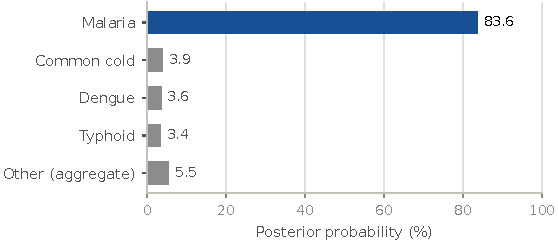
\includegraphics[width=\columnwidth]{fig_differential.pdf}
\caption{The confidence-ranked differential of Table~\ref{tab:diff}. The
leading condition is drawn in the accent tone and the remaining candidates in
grey. A dominant leading bar, as here, indicates a confident call; a near-tie
between the first two bars would instead invite a further follow-up
question.}
\label{fig:diff}
\end{figure}

%---------------------------------------------------------------- FIG TRACE
\begin{figure}[tb]
\centering
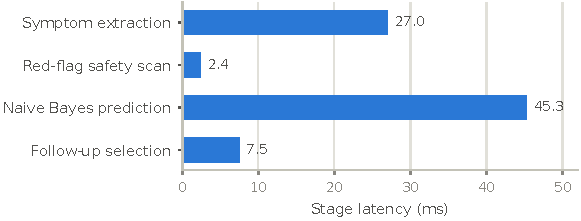
\includegraphics[width=\columnwidth]{fig_trace.pdf}
\caption{Per-stage latency for the clarifying turn of
Table~\ref{tab:trace}. Prediction dominates the turn, while the red-flag scan
which precedes it costs 2.4\,ms. The four stages together account for
82.2\,ms.}
\label{fig:trace}
\end{figure}

%---------------------------------------------------------------- FIG TRACESS
\begin{figure}[tb]
\centering
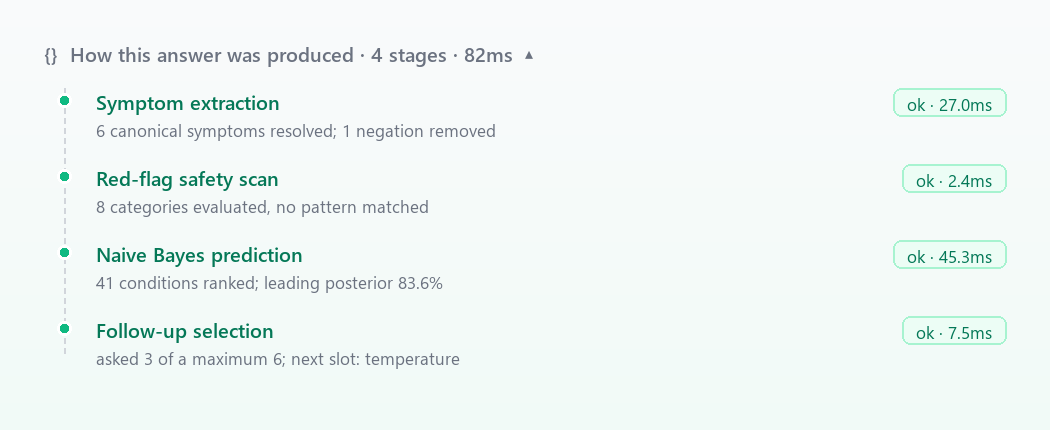
\includegraphics[width=\columnwidth]{screenshot_trace.png}
\caption{The trace as the user sees it, expanded. Each stage carries its
status, its measured time and a short note on what it did, and the stages
appear in execution order, so the position of the red-flag scan ahead of the
prediction is open to inspection on every turn.}
\label{fig:tracess}
\end{figure}

\subsection{Guided Intake in Practice}

The structured intake is what turns a single message into a short
consultation. Table~\ref{tab:prompts} lists the six prompts which the system
draws on, each of which ships with quick-reply options, so that the user can
answer with a tap rather than with free text. Clinical slots and
model-selected discriminating symptoms are interleaved, so the conversation
covers both the context (how long, how severe, getting better or worse) and
the specific distinctions needed to separate the leading candidates. Several
of the answers feed back into the feature vector and sharpen the differential
before any assessment is shown.

%---------------------------------------------------------------- TABLE V
\begin{table}[t]
\caption{Top-ranked conditions for the example symptom set}
\label{tab:diff}
\centering
\footnotesize
\begin{tabular}{@{}l r@{}}
\toprule
\textbf{Condition} & \textbf{Probability (\%)}\\
\midrule
Malaria            & 83.6\\
Common cold        & 3.9\\
Dengue             & 3.6\\
Typhoid            & 3.4\\
Other (aggregate)  & 5.5\\
\bottomrule
\end{tabular}
\end{table}

%---------------------------------------------------------------- TABLE VI
\begin{table}[t]
\caption{Representative per-turn processing trace (clarifying turn)}
\label{tab:trace}
\centering
\footnotesize
\begin{tabular}{@{}l c r@{}}
\toprule
\textbf{Stage} & \textbf{Status} & \textbf{Time (ms)}\\
\midrule
Symptom extraction     & \code{ok} & 27.0\\
Red-flag safety scan   & \code{ok} & 2.4\\
Naive Bayes prediction & \code{ok} & 45.3\\
Follow-up selection    & \code{ok} & 7.5\\
\bottomrule
\end{tabular}
\end{table}

%---------------------------------------------------------------- TABLE VII
\begin{table}[t]
\caption{Follow-up prompts used by the guided intake}
\label{tab:prompts}
\centering
\footnotesize
\begin{tabular}{@{}p{0.17\linewidth} p{0.30\linewidth} p{0.38\linewidth}@{}}
\toprule
\textbf{Slot} & \textbf{Prompt} & \textbf{Example options}\\
\midrule
Duration & How long have you felt this way? &
$<$1 day; 1--3 days; $\sim$a week; $>$2 weeks\\[1pt]
Intensity & How intense is it overall? &
Mild; moderate; severe\\[1pt]
Trend & Is it improving or worsening? &
Better; worse; about the same\\[1pt]
Temperature & Have you measured your temperature? &
$<$100; 100--102; $>$102\,\degF; not measured\\[1pt]
Exposure & Anything relevant recently? &
Travel; sick contact; new food; none\\[1pt]
Appetite/sleep & How are appetite and sleep? &
Normal; eating less; sleeping poorly\\
\bottomrule
\end{tabular}
\end{table}

%---------------------------------------------------------------- DISCUSSION
\section{Discussion}

\subsection{The Language Model as an Optional Layer}

Confining the language model to extraction and phrasing has a practical
payoff: the system behaves in the same way whether or not a key is present.
With a model configured, symptom extraction copes with unusual phrasing and
the explanations read more naturally; without one, a fuzzy matcher over the
canonical vocabulary takes over. In our measurements the fallback path still
recovered the correct symptoms for the running example, while removing a
network round-trip from every turn, and this is the reason why the safety and
ranking guarantees never depend on the availability of a model.

\subsection{Why Naive Bayes}

The choice of a Multinomial Naive Bayes classifier is deliberate rather than
incidental. A single prediction costs of the order of $O(n|\mathcal{C}|)$
operations, roughly $87 \times 41$ here. Thus it completes in well under a
millisecond, and the per-turn latency is left dominated by symptom
extraction. More importantly, the log-linear form of~(1) makes each prediction
attributable to individual symptoms, so that the reason for a ranking can be
stated plainly. A deep model might well raise the raw accuracy, but it would
do so at the cost of far more training data and of the transparency which the
application is built around.

\subsection{Scalability and Extensibility}

Extending the coverage is a local operation. Adding a condition means
retraining the classifier, adding one knowledge-base article which is
re-embedded into the index, and appending one Ayurvedic entry. Retrieval uses
approximate nearest neighbours, so it scales sub-linearly with the size of
the corpus, and the cost of prediction grows only linearly with the number of
conditions. Each request is, moreover, self-contained apart from the small
session row. Hence the backend is well suited to horizontal scaling behind a
load balancer, which we identify as a deployment step for future work.

%---------------------------------------------------------------- LIMITS
\section{Limitations and Future Work}

The most significant limitation concerns the data. A synthetic training set
makes the predictions educational rather than clinical, and re-training on
validated cohorts, with per-condition accuracy and $F_1$ reported, is the
clear next step. The language model is optional in the present build; a
configured key improves extraction and phrasing, but it alters none of the
safety guarantees. We intend further to expand both the retrieval corpus and
the Ayurvedic repository, with a citation attached to every passage, to
containerise the services for horizontal scaling, to add an authenticated
clinician-review path with an explicit human-in-the-loop escalation, and to
introduce an automated red-flag test suite alongside a clinician-rated study
of the quality of the answers. The latencies we report were obtained on a
single development machine with a warm cache, and they therefore indicate
responsiveness rather than throughput under load. The safety evaluation is so
far qualitative; a labelled corpus of emergency and non-emergency messages is
needed before sensitivity and specificity can be reported. On the ethical
side, the system does not diagnose, it never names a drug or a dose, it keeps
sessions on the user's device, and it surfaces a persistent disclaimer.

%---------------------------------------------------------------- CONCLUSION
\section{Conclusion}

Arogya AI demonstrates that a safe and transparent early-guidance assistant
can be built by treating the language model as an optional component rather
than as the centre of the system. A deterministic red-flag check guards every
turn, a Naive Bayes classifier provides an explainable and probability-ranked
differential, retrieval keeps the explanations grounded, and a curated
Ayurvedic layer adds culturally relevant guidance. The prototype is
responsive, private and robust to a missing model key, and it compares
favourably with the usual families of tools on conversation, safety,
transparency and holistic care. It remains an aid to understanding, and not a
substitute for professional medical care.

%---------------------------------------------------------------- REFS
\begin{thebibliography}{20}
\footnotesize

\bibitem{shortliffe}
E. H. Shortliffe and M. J. Sep\'{u}lveda, ``Clinical decision support in the
era of artificial intelligence,'' \textit{JAMA}, vol.~320, no.~21,
pp.~2199--2200, 2018.

\bibitem{semigran}
H. L. Semigran, J. A. Linder, C. Gidengil, and A. Mehrotra, ``Evaluation of
symptom checkers for self diagnosis and triage: audit study,''
\textit{BMJ}, vol.~351, h3480, 2015.

\bibitem{ayers}
J. W. Ayers \textit{et al.}, ``Comparing physician and artificial
intelligence chatbot responses to patient questions posted to a public social
media forum,'' \textit{JAMA Intern. Med.}, vol.~183, no.~6, pp.~589--596,
2023.

\bibitem{singhal}
K. Singhal \textit{et al.}, ``Large language models encode clinical
knowledge,'' \textit{Nature}, vol.~620, no.~7972, pp.~172--180, 2023.

\bibitem{thiru}
A. J. Thirunavukarasu \textit{et al.}, ``Large language models in medicine,''
\textit{Nat. Med.}, vol.~29, pp.~1930--1940, 2023.

\bibitem{nori}
H. Nori \textit{et al.}, ``Capabilities of GPT-4 on medical challenge
problems,'' \textit{arXiv:2303.13375}, 2023.

\bibitem{lewis}
P. Lewis \textit{et al.}, ``Retrieval-augmented generation for
knowledge-intensive NLP tasks,'' in \textit{Proc. NeurIPS}, vol.~33, 2020,
pp.~9459--9474.

\bibitem{gao}
Y. Gao \textit{et al.}, ``Retrieval-augmented generation for large language
models: A survey,'' \textit{arXiv:2312.10997}, 2023.

\bibitem{xiong}
G. Xiong \textit{et al.}, ``Benchmarking retrieval-augmented generation for
medicine,'' \textit{arXiv:2402.13178}, 2024.

\bibitem{vaswani}
A. Vaswani \textit{et al.}, ``Attention is all you need,'' in \textit{Proc.
NeurIPS}, vol.~30, 2017, pp.~5998--6008.

\bibitem{bert}
J. Devlin, M.-W. Chang, K. Lee, and K. Toutanova, ``BERT: Pre-training of
deep bidirectional transformers for language understanding,'' in
\textit{Proc. NAACL-HLT}, 2019, pp.~4171--4186.

\bibitem{sbert}
N. Reimers and I. Gurevych, ``Sentence-BERT: Sentence embeddings using
Siamese BERT-networks,'' in \textit{Proc. EMNLP-IJCNLP}, 2019,
pp.~3982--3992.

\bibitem{sklearn}
F. Pedregosa \textit{et al.}, ``Scikit-learn: Machine learning in Python,''
\textit{J. Mach. Learn. Res.}, vol.~12, pp.~2825--2830, 2011.

\bibitem{topol}
E. J. Topol, ``High-performance medicine: the convergence of human and
artificial intelligence,'' \textit{Nat. Med.}, vol.~25, pp.~44--56, 2019.

\bibitem{rajkomar}
A. Rajkomar, J. Dean, and I. Kohane, ``Machine learning in medicine,''
\textit{N. Engl. J. Med.}, vol.~380, pp.~1347--1358, 2019.

\bibitem{thamma}
S. R. Thamma, ``Agentic AI for clinical decision support: real-time
diagnosis, triage, and treatment planning,'' \textit{Int. J. Sci. Res. Sci.
Eng. Technol.}, vol.~12, no.~3, pp.~428--433, 2025.

\bibitem{patel}
H. Patel, D. Sathwara, V. Maheshwari, and D. Joshi, ``Harnessing artificial
intelligence for the future of precision medicine,'' \textit{Biopress J.
Comput. Life Sci.}, vol.~1, no.~4, 2025.

\bibitem{khan}
S. Khan and M. R. Ghalib, ``A Naive-Bayes approach for disease diagnosis with
analysis of disease type and symptoms,'' \textit{Int. J. Appl. Eng. Res.},
vol.~10, no.~11, pp.~29005--29014, 2015.

\bibitem{alqarni}
S. S. Al-qarni and A. Algarni, ``Disease prediction from symptom descriptions
using deep learning and NLP,'' \textit{Int. J. Adv. Comput. Sci. Appl.},
vol.~16, no.~5, pp.~416--426, 2025.

\bibitem{spec}
R. Shrivastava and A. Rai, ``Arogya AI: agentic disease prediction with
Ayurvedic recommendations,'' Course Project Specification, Dept. CSE, Vellore
Institute of Technology, Vellore, India, 2025.

\end{thebibliography}

\end{document}
